\documentclass[10pt,a4paper,landscape]{article}
\usepackage{multicol}
\usepackage{calc}
\usepackage{ifthen}
\usepackage[landscape]{geometry}
\usepackage{hyperref}

\usepackage[utf8]{inputenc}

% Fuentes (Fira Sans)
\usepackage[T1]{fontenc}
\usepackage[sfdefault,scaled=.85]{FiraSans}
\usepackage{newtxsf}
\usepackage[scaled=.85]{FiraMono}

% TikZ for UML

\usepackage{tikz-uml}

% Listings for code

\usepackage{listings}
\lstset{basicstyle=\ttfamily\footnotesize,breaklines=true}
\lstset{literate=   % listings config
  {á}{{\'a}}1 {é}{{\'e}}1 {í}{{\'i}}1 {ó}{{\'o}}1 {ú}{{\'u}}1
  {Á}{{\'A}}1 {É}{{\'E}}1 {Í}{{\'I}}1 {Ó}{{\'O}}1 {Ú}{{\'U}}1
  {à}{{\`a}}1 {è}{{\`e}}1 {ì}{{\`i}}1 {ò}{{\`o}}1 {ù}{{\`u}}1
  {À}{{\`A}}1 {È}{{\'E}}1 {Ì}{{\`I}}1 {Ò}{{\`O}}1 {Ù}{{\`U}}1
  {ä}{{\"a}}1 {ë}{{\"e}}1 {ï}{{\"i}}1 {ö}{{\"o}}1 {ü}{{\"u}}1
  {Ä}{{\"A}}1 {Ë}{{\"E}}1 {Ï}{{\"I}}1 {Ö}{{\"O}}1 {Ü}{{\"U}}1
  {â}{{\^a}}1 {ê}{{\^e}}1 {î}{{\^i}}1 {ô}{{\^o}}1 {û}{{\^u}}1
  {Â}{{\^A}}1 {Ê}{{\^E}}1 {Î}{{\^I}}1 {Ô}{{\^O}}1 {Û}{{\^U}}1
  {œ}{{\oe}}1 {Œ}{{\OE}}1 {æ}{{\ae}}1 {Æ}{{\AE}}1 {ß}{{\ss}}1
  {ű}{{\H{u}}}1 {Ű}{{\H{U}}}1 {ő}{{\H{o}}}1 {Ő}{{\H{O}}}1
  {ç}{{\c c}}1 {Ç}{{\c C}}1 {ø}{{\o}}1 {å}{{\r a}}1 {Å}{{\r A}}1
  {€}{{\EUR}}1 {£}{{\pounds}}1 {ñ}{{\~{n}}}1
}

% Multiple cols/rows

\usepackage{multirow}

% Checkmarks

\usepackage{amssymb}

% To make this come out properly in landscape mode, do one of the following
% 1.
%  pdflatex latexsheet.tex
%
% 2.
%  latex latexsheet.tex
%  dvips -P pdf  -t landscape latexsheet.dvi
%  ps2pdf latexsheet.ps


% If you're reading this, be prepared for confusion.  Making this was
% a learning experience for me, and it shows.  Much of the placement
% was hacked in; if you make it better, let me know...


% 2008-04
% Changed page margin code to use the geometry package. Also added code for
% conditional page margins, depending on paper size. Thanks to Uwe Ziegenhagen
% for the suggestions.

% 2006-08
% Made changes based on suggestions from Gene Cooperman. <gene at ccs.neu.edu>


% To Do:
% \listoffigures \listoftables
% \setcounter{secnumdepth}{0}


% This sets page margins to .5 inch if using letter paper, and to 1cm
% if using A4 paper. (This probably isn't strictly necessary.)
% If using another size paper, use default 1cm margins.
\ifthenelse{\lengthtest { \paperwidth = 11in}}
	{ \geometry{top=.5in,left=.5in,right=.5in,bottom=.5in} }
	{\ifthenelse{ \lengthtest{ \paperwidth = 297mm}}
		{\geometry{top=1cm,left=1cm,right=1cm,bottom=1cm} }
		{\geometry{top=1cm,left=1cm,right=1cm,bottom=1cm} }
	}

% Turn off header and footer
\pagestyle{empty}
 

% Redefine section commands to use less space
\makeatletter
\renewcommand{\section}{\@startsection{section}{1}{0mm}%
                                {-1ex plus -.5ex minus -.2ex}%
                                {0.5ex plus .2ex}%x
                                {\normalfont\large\bfseries}}
\renewcommand{\subsection}{\@startsection{subsection}{2}{0mm}%
                                {-1explus -.5ex minus -.2ex}%
                                {0.5ex plus .2ex}%
                                {\normalfont\normalsize\bfseries}}
\renewcommand{\subsubsection}{\@startsection{subsubsection}{3}{0mm}%
                                {-1ex plus -.5ex minus -.2ex}%
                                {1ex plus .2ex}%
                                {\normalfont\small\bfseries}}
\makeatother

% Define BibTeX command
\def\BibTeX{{\rm B\kern-.05em{\sc i\kern-.025em b}\kern-.08em
    T\kern-.1667em\lower.7ex\hbox{E}\kern-.125emX}}

% Don't print section numbers
\setcounter{secnumdepth}{0}


\setlength{\parindent}{0pt}
\setlength{\parskip}{0pt plus 0.5ex}


% -----------------------------------------------------------------------

\begin{document}

\raggedright
\footnotesize
\begin{multicols}{3}


% multicol parameters
% These lengths are set only within the two main columns
%\setlength{\columnseprule}{0.25pt}
\setlength{\premulticols}{1pt}
\setlength{\postmulticols}{1pt}
\setlength{\multicolsep}{1pt}
\setlength{\columnsep}{2pt}


\tikzumlset{font=\footnotesize}

\begin{center}
     \Large{\textbf{PDOO temas 1, 2 y 3}} \\
\end{center}

\section{Conceptos básicos}

\subsection{Especificadores de acceso}

\subsubsection{Java}

\begin{tabular}{cccc}
\multirow{2}{*}{Visible en} & \multicolumn{2}{c}{Mismo paquete} & Otro paquete
  \\
                            & Clase & Otra & Otra \\
  private & \checkmark & & \\
  package & \checkmark & \checkmark & \\
  protected & \checkmark & \checkmark & \\
  public & \checkmark & \checkmark & \checkmark \\
\end{tabular}

\subsubsection{Ruby}

\begin{tabular}{cccc}
Visible en & Desde el propio objeto & Clase & Otra\\
  private & \checkmark & & \\
  protected & \checkmark & \checkmark & \\
  public & \checkmark & \checkmark & \checkmark \\
\end{tabular}

\subsection{Especificadores de acceso (herencia)}

\subsubsection{Java}

\begin{tabular}{ccc}
\multirow{2}{*}{Visible en} & \multicolumn{2}{c}{Subclase}\\
                            & Mismo paquete & Otro paquete\\
  private &  & \\
  package & \checkmark \\
  protected & \checkmark & \checkmark\\
  public & \checkmark & \checkmark\\
\end{tabular}

\subsubsection{Ruby}

\begin{tabular}{ccc}
\multirow{2}{*}{Visible en}
                            & {El mismo objeto en } & {Cualquier objeto de}\\
                            & la subclase (self) & la subclase\\

  private & \checkmark   & \\
  protected & \checkmark & \checkmark\\
  public & \checkmark & \checkmark\\
\end{tabular}


En Ruby, los métodos \textit{protected} solo pueden llamarse desde un método de instancia. Además, pueden ser llamados únicamente desde una instancia de la clase que lo define, o de una subclase suya.

\section{Diagramas UML}

\subsection{Diagramas de clases}

\begin{tikzpicture}[]
  \umlclass{Nombre$^{multiplicidad}$}{
    [visibilidad] nombreAtributo [:tipo[multiplicidad]][=valorInicial] \\
    $\vdots$ \\
  }{
    [visibilidad] nombreMétodo ([lista parámetros])[:tipo retorno] \\
    $\vdots$ \\
  }
\end{tikzpicture}

\hspace{4em}
\verb!+! Pública \quad
\verb!-!  Privada \quad
\verb!~! Paquete \quad
\verb!#! Protegida \quad

 \subsection{Diagramas de secuencia}
Los argumentos de
 los fragmentos de interacción descritos a continuación se indican dentro, en un recuadro.

\begin{tabular}{@{}ll@{}}
  alt & Se ejecuta si se cumple la condición \\
  break & Se ejecuta si se cumple la condición y no se continúa \\
  loop & Se realiza arg veces el fragmento \\
  opt & Como alt pero con un solo fragmento \\
\end{tabular}
 
\subsection{Diagramas de comunicación}

Tipos de enlace (objetoX envía mensaje a objetoY):

\begin{tabular}{@{}l@{}l@{}l@{}}
Global \ & \texttt{G}    & \ \  El ámbito de objetoY es superior al de objetoX \\
Asociación \  &  \texttt{A}  & \ \ Existe una relación fuerte y duradera \\
Parámetro \ & \texttt{P} & \ \ objetoY es pasado como parámetro de objetoX \\
  Local \ & \texttt{L}  & \ \ objetoY es referenciado en un método de objetoX \\
  Self \ & \texttt{S} & \ \ objetoX siempre se conoce a sí mismo \\
\end{tabular}
\vspace{.5em}

Estructuras de control:

\begin{tabular}{@{}l@{}l@{}l@{}}
[condición] \ \ & Selectivas. \\
*[condición] \ \ & Iterativas. \\
\end{tabular}

\section{Herencia}

Relación \textit{es-un}. Diferente a composición.
\subsection{Métodos y atributos}

\subsubsection{Java}

$\diamond$ Los atributos privados de instancia se 'heredan' (al crearse en el constructor), pero no son accesibles desde la subclase. Igual en Ruby.

$\diamond$ Los métodos de clase se heredan, pero quedan ligados a la clase donde se definen. Pueden sobreescribirse, pero lo que hacemos en realidad es ocultar el antiguo (NO @Override). Sin embargo, no se comportan de forma polimórfica. No se pueden redefinir métodos \textit{final}.

$\diamond$ Si modificamos un atributo de clase, la modificación será visible desde la clase donde se modifica hacia abajo en el árbol de herencia, siempre y cuando en la clase donde modificamos definamos un nuevo método static para consultarlo. En otro caso, utilizará el consultor static de la clase padre, que está ligado a ella, por lo que no imprimirá el valor modificado. Los atributos de clase en realidad no se sobreescriben, sino que se ocultan. 

$\diamond$ Los constructores se heredan siempre que no tengan argumentos. En otro caso, hay que definirlos explícitamente. 

$\diamond$ Se pueden modificar métodos que se redefinen, en cuanto a tipo o número de parámetros. En realidad estaríamos sobrecargando el método, sin ocultar el de la clase padre. Se puede cambiar el tipo de retorno, siempre que sea una subclase del original. También se puede cambiar la visibilidad, siempre que sea menos restrictiva que la del original.

\subsubsection{Ruby}

$\diamond$ Los atributos de instancia de la clase no se heredan, cada clase tiene el suyo. Sin embargo, los métodos de clase sí se heredan. Se pueden sobreescribir. Hay que poner el require\_relative para heredar. Si se modifica un atributo de clase, se modifica en todo el árbol de herencia.

$\diamond$ Se hereda el constructor.

$\diamond$ Se pueden modificar los métodos que se sobreescriben, en cuanto al número o el tipo de parámetros. No existe la sobrecarga, por lo que al hacer eso, se 'oculta' el método antiguo.

\subsection{Pseudovariable super}

Permite invocar métodos de la clase padre. En Java, puede llamarse de dos formas:

\begin{tabular}{@{}l@{}l@{}l@{}}
	super.met1() \ \ & Invoca el método 'met1' de la clase padre.\\
	
	super(args) \ \ & Invoca el constructor de la clase padre con los argumentos \textit{args}.\\
	&  Únicamente en la primera línea del constructor.\\
\end{tabular}

En Ruby, \textit{super} solo puede llamar al método de la clase padre al que sobreescribe. Tiene tres variantes:

\begin{tabular}{@{}l@{}l@{}l@{}}
	super \ \ & Invoca con los mismos argumentos.\\
	
	super() \ \ & Invoca sin argumentos (¡OJO!).\\
	super(args) \ \ &  Invoca con los argumentos \textit{args}.\\
\end{tabular}

\subsection{Clases abstractas e interfaces}

\textbf{Clases abstractas.} Palabra clave \textit{abstract}. Tienen al menos un método sin implementar, también marcado como \textit{abstract}.

\textbf{Interfaces.} No son clases. Palabra clave \textit{interface}. Son una colección de métodos públicos (\textit{default}, \textit{static}, o implícitamente \textit{abstract}) y de constantes (implícitamente \textit{public}, \textit{static} y \textit{final}).

En ambos casos, si una clase hereda o implementa, debe definir todos los métodos que queden sin definir (excepto \textit{default}). De lo contrario, esta clase debe marcarse como \textit{abstract}. No se pueden instanciar. No existen en Ruby.

Se permite herencia múltiple entre inferfaces. Los métodos \textit{default} pueden sobreescribirse. Los métodos \textit{static} se pueden llamar desde otros métodos \textit{static} o \textit{default} de la interfaz, y también desde fuera. No se pueden sobreescribir (no se heredan).

Si una clase implementa una o varias interfaces (ej: In),  y hay conflicto de nombres al llamar a un método de esta última, debe ponerse \textit{In.super.metodo()}.

\section{Polimorfismo}

Es necesario \textit{downcast} para que cuadre el tipo estático. También en llamada a métodos o al añadir a un ArrayList.

\lstinputlisting[language=Java]{poli.java}

\end{multicols}
\end{document}
